\chapter{Mapping}

\section{Method}
This chapter decribes the process of building a separate static and a dynamic map (containing non-moving and moving obstacles, respectively) based on radial distance measurements (in this case provided by a LIDAR). Isolating the static and the moving obstacles from each other has its difficulties but also its advantages. First of all, the implemented local track planner calculates safer, more optimized paths if it is informed of both the static and the dynamic obstacles along the path. Secondly, \href{https://en.wikipedia.org/wiki/Simultaneous_localization_and_mapping}{SLAM} (Simultaneous localization and mapping) algorithms work better if the their input contains only static objects in the space, because they build an internal map of the world. Passing detections of moving obstacles to a SLAM algorithm may lead to worse localization quality, as they may ruin this map.

As a first subtask of the mapping project, I checked if any implementation is avaiable already, that can handle dynamic objects. The only possible candidate was \href{http://wiki.ros.org/gmapping}{gmapping}, which is a popular ROS package, used in a wide variety of applications that require map-building and localization. Its SLAM algorithm takes LIDAR measurements as its input and generates an occupancy grid (a 2D map) of the car's environment. By using this map it is able to make corrections to the car's odometry-based position and orientation, which is usually inaccurate. I tried out the package, and the result maps were promising, the generated map was insensitive to the car's longitudinal movements and its rotations. But unfortunately, gmapping's SLAM does not support dynamic objects. See \autoref{chap:static_map} for further details. Therefore, gmapping could not be used as the producer of the static map. But that didn't mean it couln't be used for its second feature, localization. Note, that the mapping implementation I made is not a SLAM algorithm, it is not able to make corrections to the car's pose. So for that purpose, I still needed the help of gmapping, which proved to be very reliable at localization. But the static map-building needed to be implemented internally.

In order to create two disjunct maps, one static and one dynamic, the key element of the process is the separation of the moving and non-moving obstacles of the measured points. After determining these two disjunct set of points, the maps can be converted to any desired or required format. Static maps are usually published as occupancy grids, while dynamic obstacles need to present information about their speed vector. Occupancy grids do not group the grid points according to their probabilities, therefore they do not know about the obstacles' borders and areas\footnote{In this project, 2D LIDARs were used, therefore the measured objects were seen as 2D shapes that have areas, not 3D objects that have volumes}. Dynamic obstacles however can be either represented as separate points with their own speed vectors, or groups of points, each groups having one speed vector. I chose the latter representation, thus publishing groups that contain a set of points (all the points, ideally) of the same obstacle. This way there is a one-to-one relationship between moving obstacles and groups. The separation and grouping methods of the mapping process is shown on diagram \ref{mapping_method}.

\tikzset{
     base_node/.style = {rectangle, rounded corners, draw=black,
                         minimum width=5cm, minimum height=1cm,
                         text centered, font=\sffamily},
  inout_node/.style   = {base_node, fill=blue!30},
  common_node/.style  = {base_node, fill=orange!15},
  dynamic_node/.style = {base_node, fill=green!30},
  static_node/.style  = {base_node, fill=red!30},
  decoration={brace},
  tuborg/.style={decorate},
  tubnode_left/.style={midway, left=2pt},
  tubnode_right/.style={midway, right=2pt}
}

\begin{figure}[!ht]
    \begin{tikzpicture}[
            node distance=1.5cm,
            every node/.style={fill=white, font=\sffamily}, align=center]
        % Node descriptions
        \node (scan)            [inout_node]                                   {Input scan};
        \node (convert_abs)     [common_node, below of=scan]                   {Convert to absolute points};
        \node (dynamic_points)  [common_node, below of=convert_abs]            {Find dynamic points};
        \node (groups)          [common_node, below of=dynamic_points]         {Make dynamic groups};
        \node (separate)        [common_node, below of=groups]                 {Separate static points from groups};
        % Dynamic nodes
        \node (speed_vectors)   [dynamic_node, below of=separate, xshift=-3cm] {Calculate speed vectors};
        \node (areas)           [dynamic_node, below of=speed_vectors]         {Calculate and validate areas};
        \node (publish_dynamic) [inout_node, below of=areas]                   {Publish dynamic obstacles};
        % Static nodes
        \node (update_map)      [static_node, below of=separate, xshift=3cm]   {Update static map};
        \node (convert_scan)    [static_node, below of=update_map]             {Remap to LIDAR scan};
        \node (publish_static)  [inout_node, below of=convert_scan]            {Publish static scan};
        % Connections
        \draw[->]           (scan) -- (convert_abs);
        \draw[->]    (convert_abs) -- (dynamic_points);
        \draw[->] (dynamic_points) -- (groups);
        \draw[->]         (groups) -- (separate);
        % Dynamic connections
        \draw[->]       (separate) -- (speed_vectors);
        \draw[->]  (speed_vectors) -- (areas);
        \draw[->]          (areas) -- (publish_dynamic);
        % Static connections
        \draw[->]       (separate) -- (update_map);
        \draw[->]     (update_map) -- (convert_scan);
        \draw[->]   (convert_scan) -- (publish_static);
        % Decorations
        \draw[tuborg, decoration={brace}] let \p1=(scan.north), \p2=(separate.south) in
            ($(\x1+3.4cm, \y1)$) -- ($(\x1+3.4cm, \y2)$) node[tubnode_right] {Separation + grouping};
        \draw[tuborg, decoration={brace}] let \p1=(speed_vectors.north), \p2=(publish_dynamic.south) in
            ($(\x1-3cm, \y2)$) -- ($(\x1-3cm, \y1)$) node[tubnode_left] {Dynamic};
        \draw[tuborg, decoration={brace}] let \p1=(update_map.north), \p2=(publish_static.south) in
            ($(\x1+3cm, \y1)$) -- ($(\x1+3cm, \y2)$) node[tubnode_right] {Static};
    \end{tikzpicture}
    \caption{Mapping method}
    \label{mapping_method}
\end{figure}

The diagram consists of 3 subgraphs - these are also marked on the diagram. The first, and most important is the separation and grouping of dynamic points. The second section describes the additional calculations that need to be done for the dynamic obstacles, and consists the documentation for the message structure definining these dynamic obstacles. The third section is about the static map that is built from the static points. The next sections are going to explain these subgraphs in detail.

\section{Separation and grouping}
This section describes the method of separating dynamic and static points of the input scan. This step is essential in the pipeline of creating two disjunct maps.

\subsection{Input scan}
The input of the mapping algorithm is a 2D LIDAR scan, consisting of radial distance measurements. Two types of LIDARs were used in the project, \href{http://www.slamtec.com/en/lidar/a1}{RPLidar A1} and \href{http://www.slamtec.com/en/lidar/a2}{RPLidar A2}.
Both types have the following specifications:

\begin{center}
    \begin{tabular}{ | c | c | }
        \hline
        Scan rate           & 10 Hz            \\
        \hline
        Sample rate         & 8000 samples/sec \\
        \hline 
        Distance resolution & 0.2 centimeters  \\
        \hline 
        Angular resolution  & 1°               \\
        \hline 
        Detection range     & 12 meters        \\
        \hline
    \end{tabular}
\end{center}

The devices proved to be reliable, and for a project of this volume, their frequencies, resolutions and ranges were adequate. Their output after each measurement sequence is an array of radial distances, that can be visualized easily using rviz.

\begin{figure}[!ht]
    \centering
    \subfloat[Gazebo simulation]
    {
        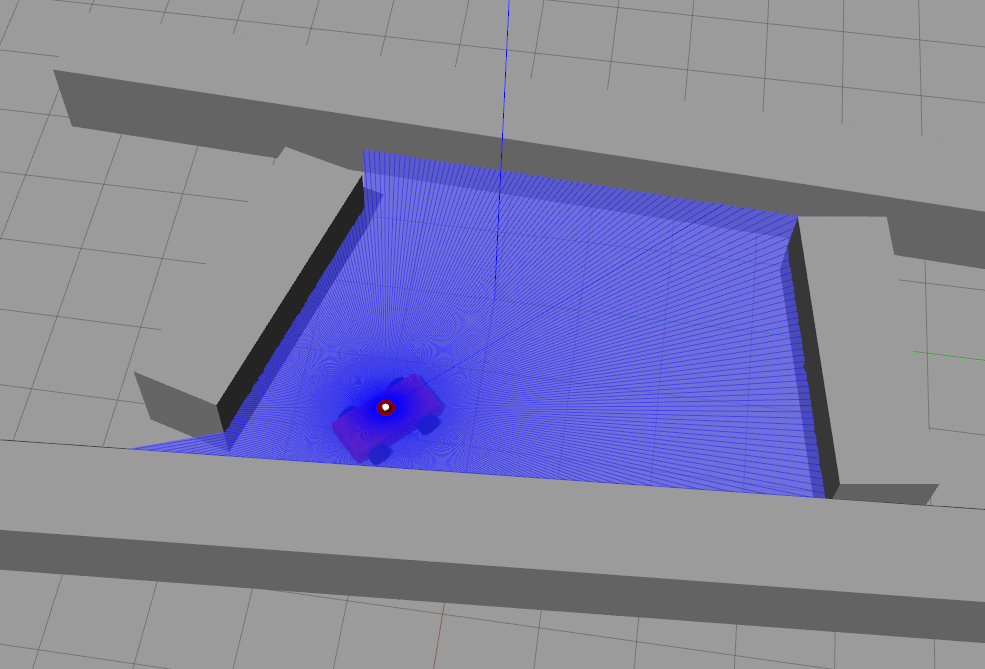
\includegraphics[height=48mm]{figures/raw/gazebo_lidar_scan.png}
        \label{gazebo_lidar_scan}
    }
    \subfloat[rviz visualization]
    {
    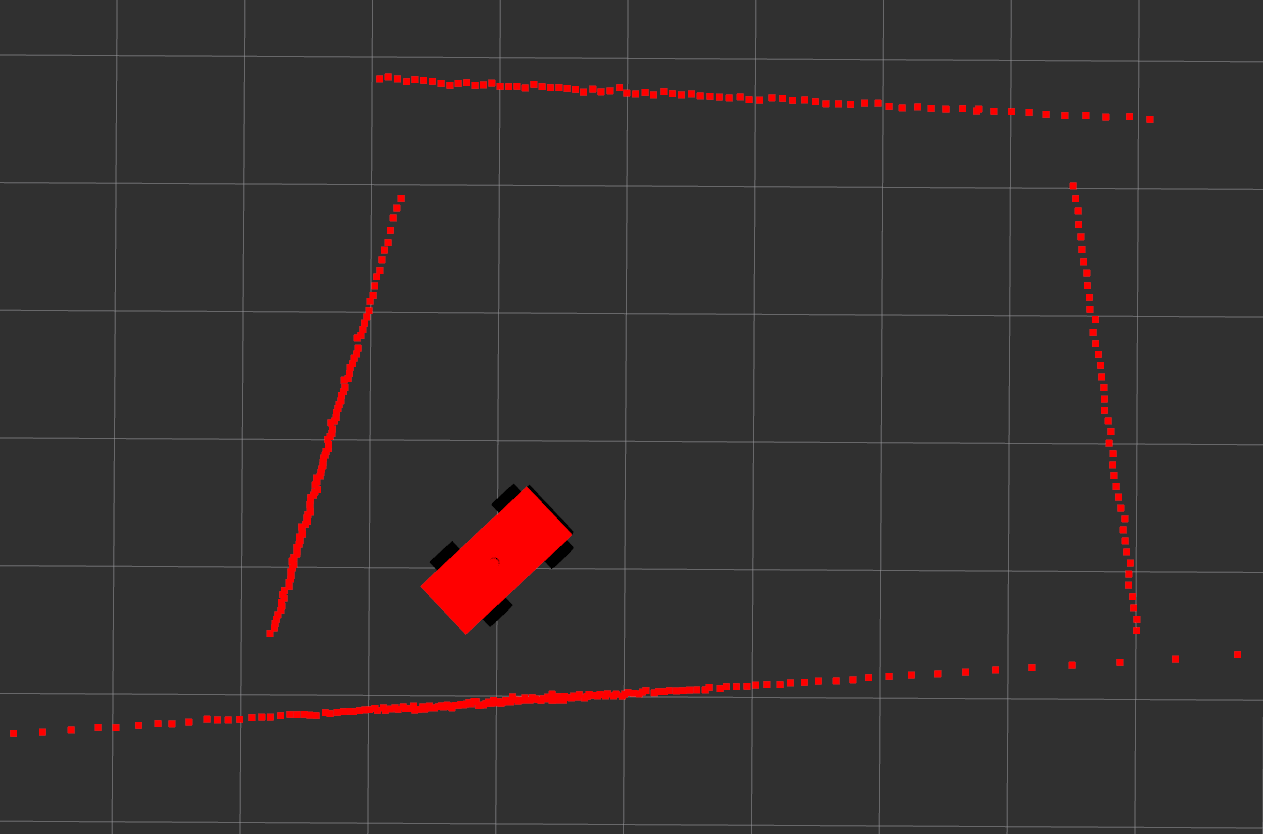
\includegraphics[height=48mm]{figures/raw/rviz_lidar_scan.png}
        \label{rviz_lidar_scan}
    }
    \caption{LIDAR scan}
    \label{lidar_scan}
\end{figure}

\subsection{Absolute points}
For static map-building, absolute points\footnote{Absolute points are not relative to the car, but to a fix base point.} are needed in the space, and static-dynamic point separation also uses absolute points, so firstly, these radial distances need to be transformed. However, the internal static map and the static-dynamic separation use different coordinate systems. In order to understand the need for this, let's take a look at figure \ref{rqt_input}.

\begin{figure}[!ht]
    \centering
    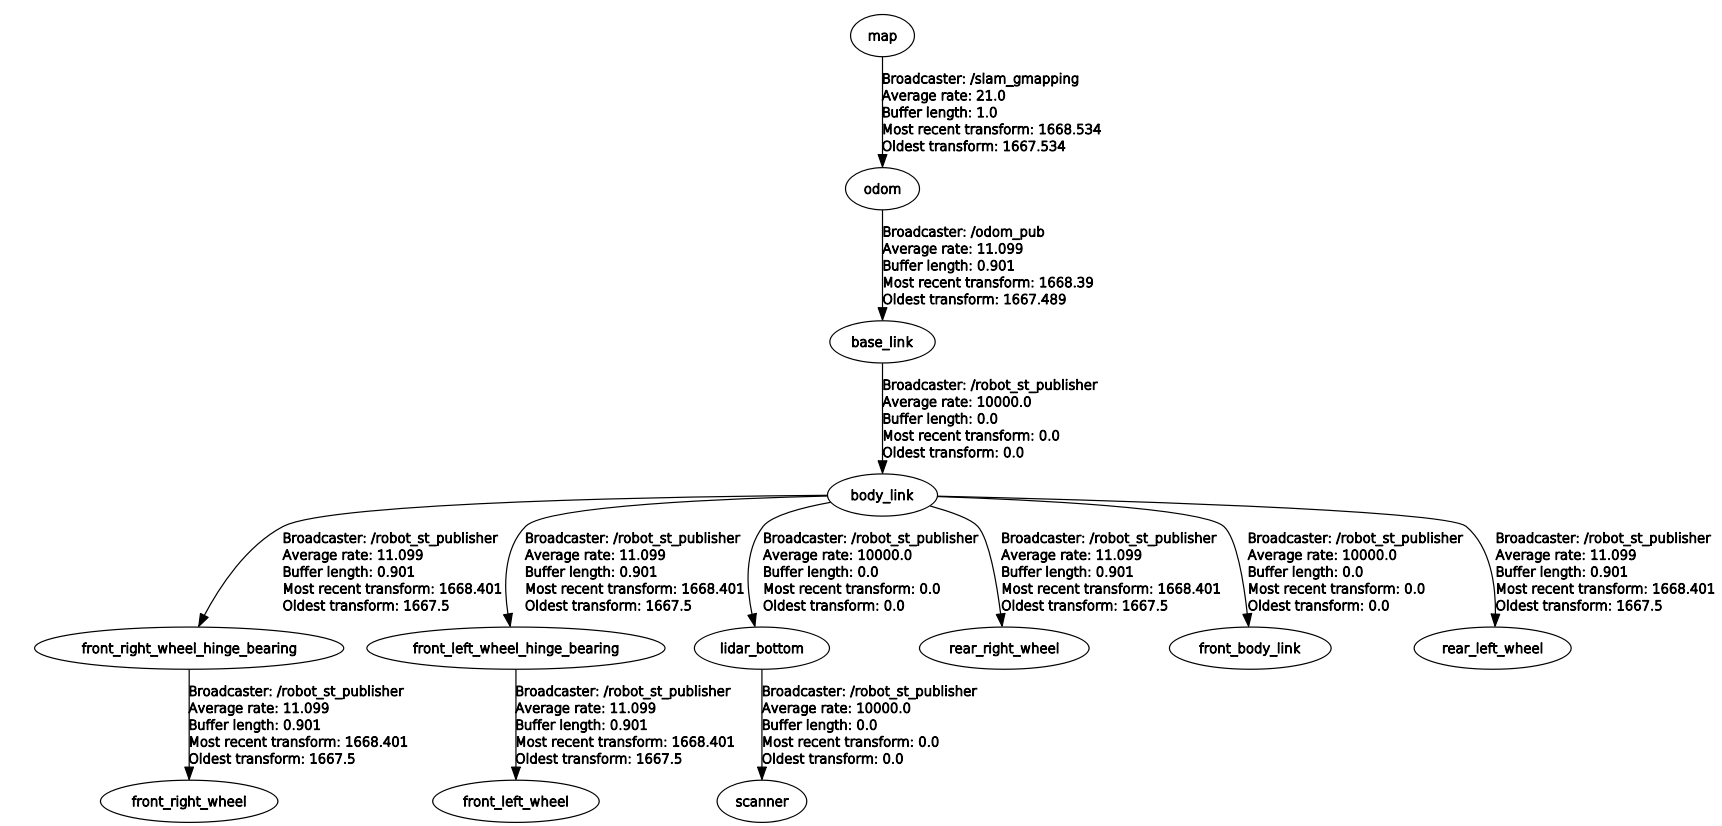
\includegraphics[height=130mm]{figures/raw/rqt_input.png}
    \caption{Coordinate frames}
    \label{rqt_input}
\end{figure}

As the figure shows, there are 3 coordinate frames that are important to the current case. The \textit{odom} frame is the car odometry's coordinate system. It is calculated from values measured on the vehicle, such as servo position and speed. The \textit{scanner} frame is the LIDAR's coordinate system. The transformation between \textit{odom} and \textit{scanner} is basically the pose of the LIDAR, relative to the car. The \textit{map} frame is the output of gmapping's localization. Basically, gmapping takes the car odometry and the LIDAR scans as its input, and corrects the odometry using SLAM. As a result the difference between frames \textit{map} and \textit{odom} will increase with time.

The internal static map in my imlpementation uses this corrected \textit{map} frame as the base for its points, so that its error is minimized. But unfortunately, the static-dynamic separation method cannot use this frame. The reason is that this frame does not get updated on every new scan, but with a much slower frequency. Therefore there are 'jumps' in the \textit{map} frame, which would cause false dynamic point detections (see \autoref{chap:dynamic_points}). To avoid this undesired situation, the static-dynamic separation uses the \textit{odom} frame as its base, which is more continuous than the \textit{map} frame.

Therefore, two transformations are needed for each input point. The transformations are calculated using \href{http://wiki.ros.org/tf}{tf}, which maintains the relationship between coordinate frames in a tree structure (see figure \ref{rqt_input}) buffered in time, and makes the transformation of points, vectors, etc possible at any desired point in time.

\subsection{Dynamic points}
\label{chap:dynamic_points}
The next step is similar to a creating a subtraction image in image processing, where subtracting two images, taken from the same position but at a different time, results in an image that amplifies the movements between the snapshots. The aim of this algorithm unit is basically the same: selecting the points from the input that are likely to be part of a moving mass. This is done by finding the points among the current measurements that have not been present in the previous ones.

This step is best explainable in practice. Let's assume that the position and orientation of the LIDAR is fix, and one object (e.g. a car) in the detected area is moving. Figure \ref{obstacle_movement} shows this situation. On the image, the pale contour represents the previous pose of the object, and the current state is blue.

\begin{figure}[!ht]
    \centering
    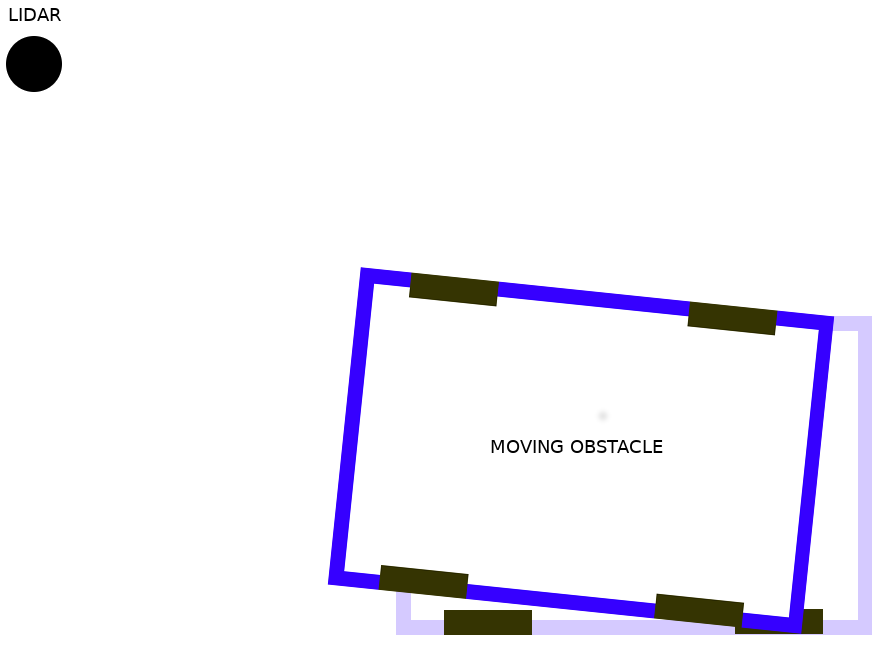
\includegraphics[height=80mm]{figures/raw/obstacle_movement.png}
    \caption{The obstacle is moving}
    \label{obstacle_movement}
\end{figure}

Figure \ref{obstacle_movement_lidar} shows how the LIDAR detects the moving object in two different timesnaps. I marked the points corresponding to the current position with red color, and the ones of the previous measurement are pale red. As it is suggested in the figure, the measurements are far from ideal, the detected points are noisy.

\begin{figure}[!ht]
    \centering
    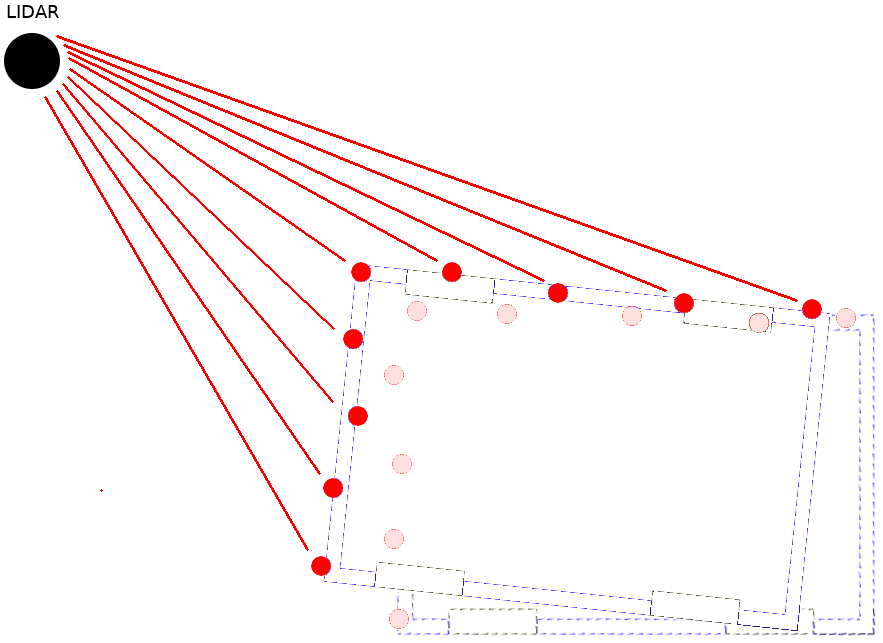
\includegraphics[height=80mm]{figures/raw/obstacle_movement_lidar.png}
    \caption{The detected points of the moving obstacle}
    \label{obstacle_movement_lidar}
\end{figure}

To understand the method of dynamic point detection, I removed the LIDAR, its virtual rays and the obstacle's contour from the image, thus leaving leaving only the measured points of the two timesnap. The result, which is basically a time-buffered array of 2D points, is presented on figure \ref{obstacle_movement_lidar_only}. The algorithm iterates through each point in the current measurement, and checks if any point in the previous measurements\footnote{The number of measurements to 'look up' is configurable.} is within its compliance radius\footnote{The compliance radius is a maximum allowed distance between measurements representing the same physical point but measured in different timesnaps. If the distance between two measurements is greater than this value, the measurements are assumed to represent different points of the space. The compliance radius is calculated for each measurement separately, and it is proportional to the distance of the LIDAR and the measured point.}.

\begin{figure}[!ht]
    \centering
    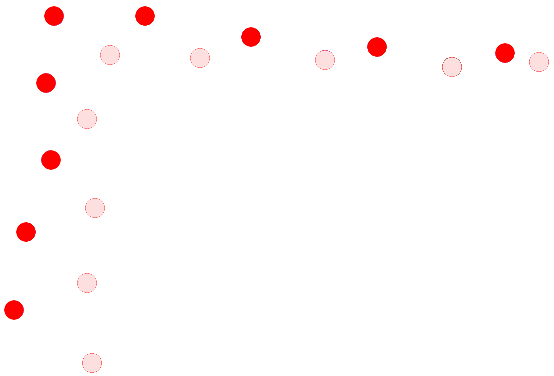
\includegraphics[height=50mm]{figures/raw/obstacle_movement_lidar_only.png}
    \caption{The detected points of the two timesnaps}
    \label{obstacle_movement_lidar_only}
\end{figure}

The measured points with their compliance radiuses are presented in figure \ref{compliance_radiuses}. The possible dynamic points, that have no points from the previous measurement within their radius, are marked with blue, and their compliance radius with yellow. The possible static points are marked with red, along with their radiuses. Note, that these points are \textit{possible} dynamic and static points. The final classification will be preceded be multiple filtering mechanisms and point grouping, but this is the base for finding dynamic objects.

\begin{figure}[!ht]
    \centering
    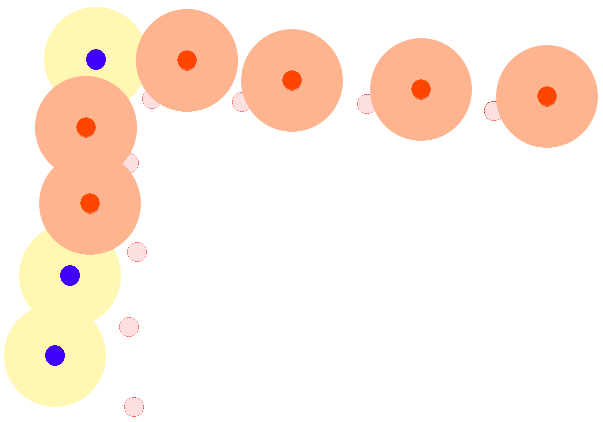
\includegraphics[height=50mm]{figures/raw/compliance_radiuses.png}
    \caption{The compliance radiuses and the dynamic points}
    \label{compliance_radiuses}
\end{figure}

Several conclusions can be drew from figure \ref{compliance_radiuses}. The one, and probably most important is that with right parameterizing (number of 'look-up' measurements, compliance radius, etc) this method amplifies the positive\footnote{Previously a distant background was detected, but now a closer object appears.} and negative\footnote{Previously a close object was detected, but now it disappears, and the distant background becomes visible.} changes of the scans. The second remark is that the method does not detect all the points of a moving object. However, due to measurement noise false detections may happen, non-moving points may be marked as dynamic. Therefore, this separation needs to be followed by several filtering and validating steps.

\subsection{Dynamic groups}


\subsection{Separation of static points and dynamic groups}


\section{Dynamic obstacles}
After the dynamic groups have been separated from the static points, additional information needs to be calculated for them, so that the local track planner algorithm can use their data for its obstacle-avoidance feature.

\subsection{Speed vectors}


\subsection{Area validation}


\subsection{Publishing dynamic obstacles}


\section{Static points}
Static points used for two separate purposes. The first one is building a static map, the second is localization with the help of gmapping.

\subsection{Static map}
\label{chap:static_map}
After separating the dynamic groups from the scan points, only the static points are left. These points do not change their positions with time\footnote{Except those obstacles that start moving only after they have already been detected as sets of static points. But these objects do not ruin the quality of the map, either.}, so they can be added to the static map.

For static map-building, gmapping has already been mentioned as a candidate, but unfortunately, its algorithm does not recognize changes in the environment. In practice, if an object has been detected and placed in its map, it will not be erased from there, even after the object has moved away. Figures \ref{gmapping_drawback_before_move} and \ref{gmapping_drawback_after_move} demonstrate the problem.

\begin{figure}[!ht]
    \centering
    \subfloat[Gazebo simulation]
    {
        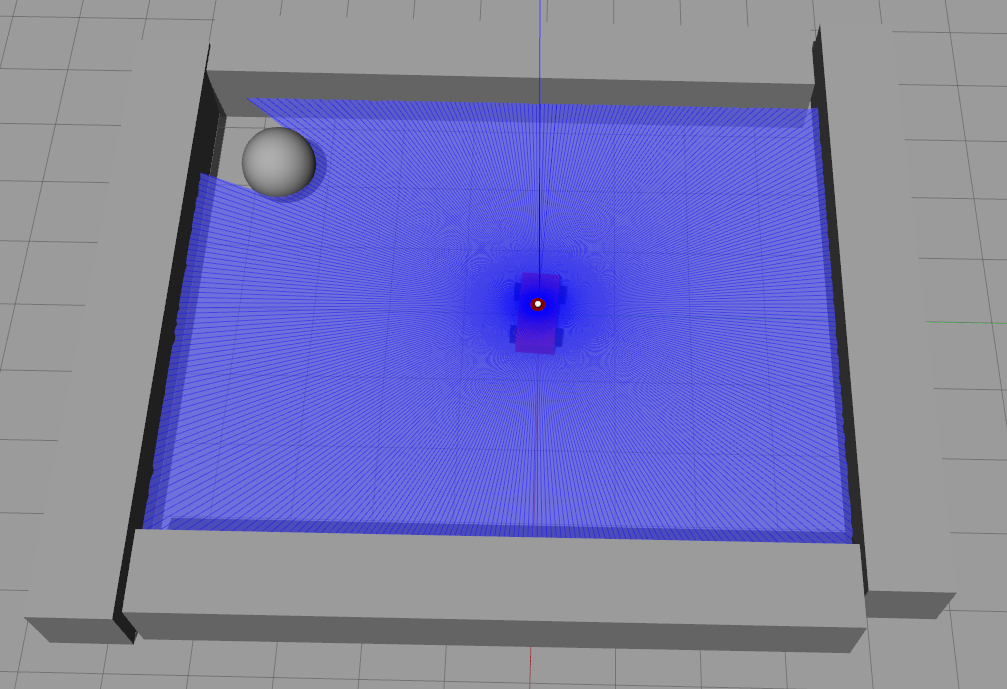
\includegraphics[height=48mm]{figures/raw/gazebo_gmapping_before_move.png}
        \label{gazebo_gmapping_before_move}
    }
    \subfloat[Map created by gmapping]
    {
    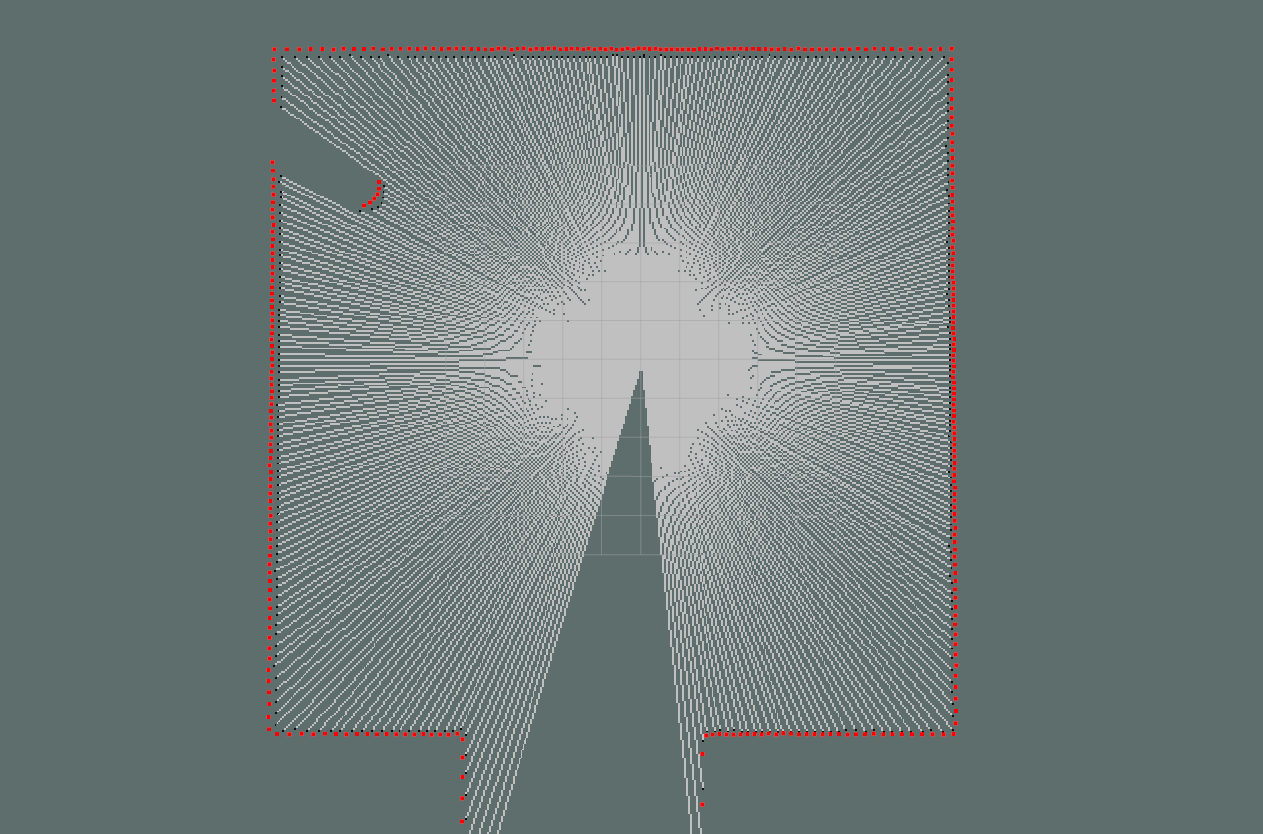
\includegraphics[height=48mm]{figures/raw/rviz_gmapping_before_move.png}
        \label{rviz_gmapping_before_move}
    }
    \caption{Initial state - ball is still}
    \label{gmapping_drawback_before_move}
\end{figure}

Figure \ref{gmapping_drawback_before_move} shows a situation where the ball is standing still. A the mapping algorithm of gmapping successfully creates a map (in the form of an occupancy grid\footnote{An occupancy grid represents a map in an evenly spaced field of probability values representing if the grid points are occupied by an obstacle}) that marks the place of the ball as occupied. However, when the ball starts moving (see figure \ref{gmapping_drawback_after_move}), the map does not change, because the algorithm cannot handle moving obstacles.

\begin{figure}[!ht]
    \centering
    \subfloat[Gazebo simulation]
    {
        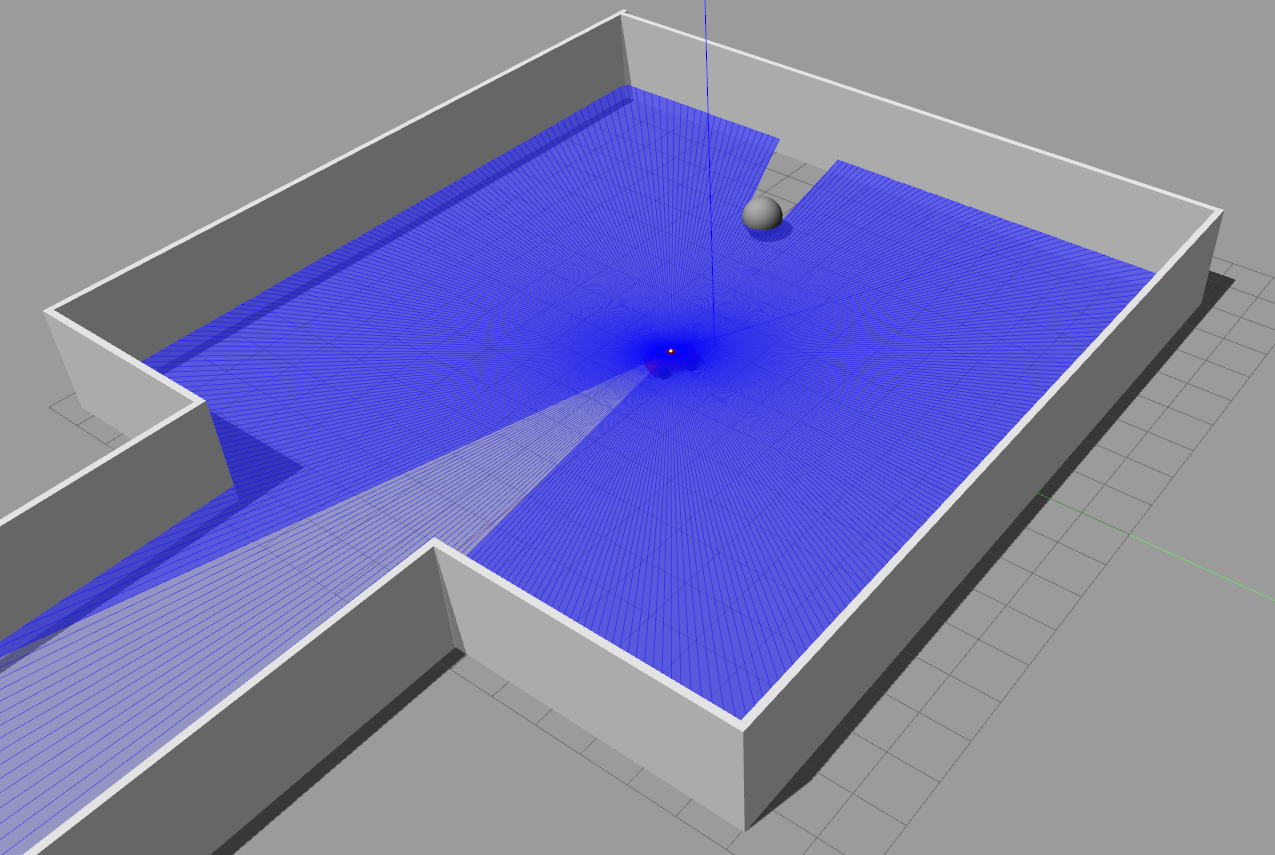
\includegraphics[height=48mm]{figures/raw/gazebo_gmapping_after_move.png}
        \label{gazebo_gmapping_after_move}
    }
    \subfloat[Map created by gmapping]
    {
        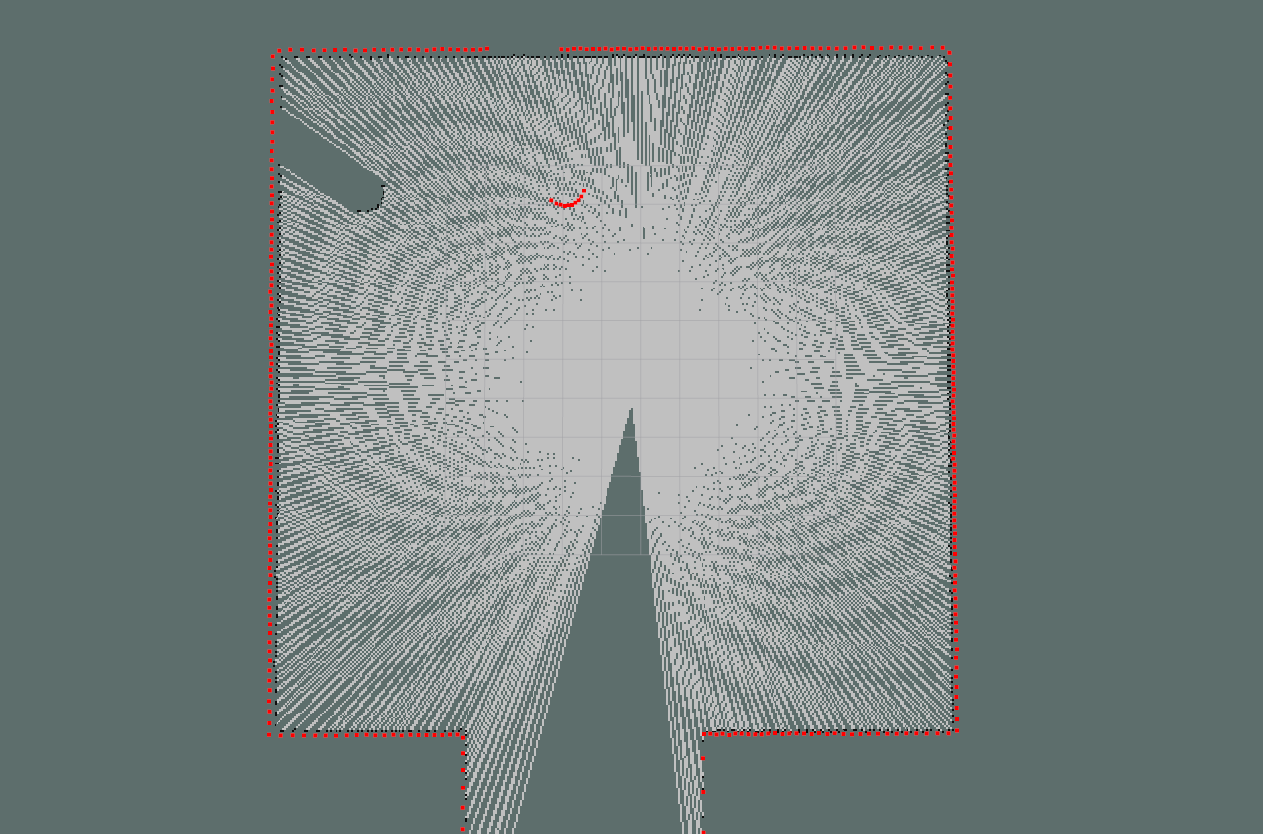
\includegraphics[height=48mm]{figures/raw/rviz_gmapping_after_move.png}
        \label{rviz_gmapping_after_move}
    }
    \caption{Moving state - ball has changed position}
    \label{gmapping_drawback_after_move}
\end{figure}


\subsection{Remapping to LIDAR scan}


\subsection{Publishing static scan}
